\section{Technology Stack}

\subsection{Architecture Overview}
Layered, decoupled three-tier design: the Next.js frontend talks only to the
REST API and the WebSocket server; all business logic, storage, and billing
live behind those interfaces (Fig.~\ref{fig:architecture}).

\begin{figure}[H]
\centering
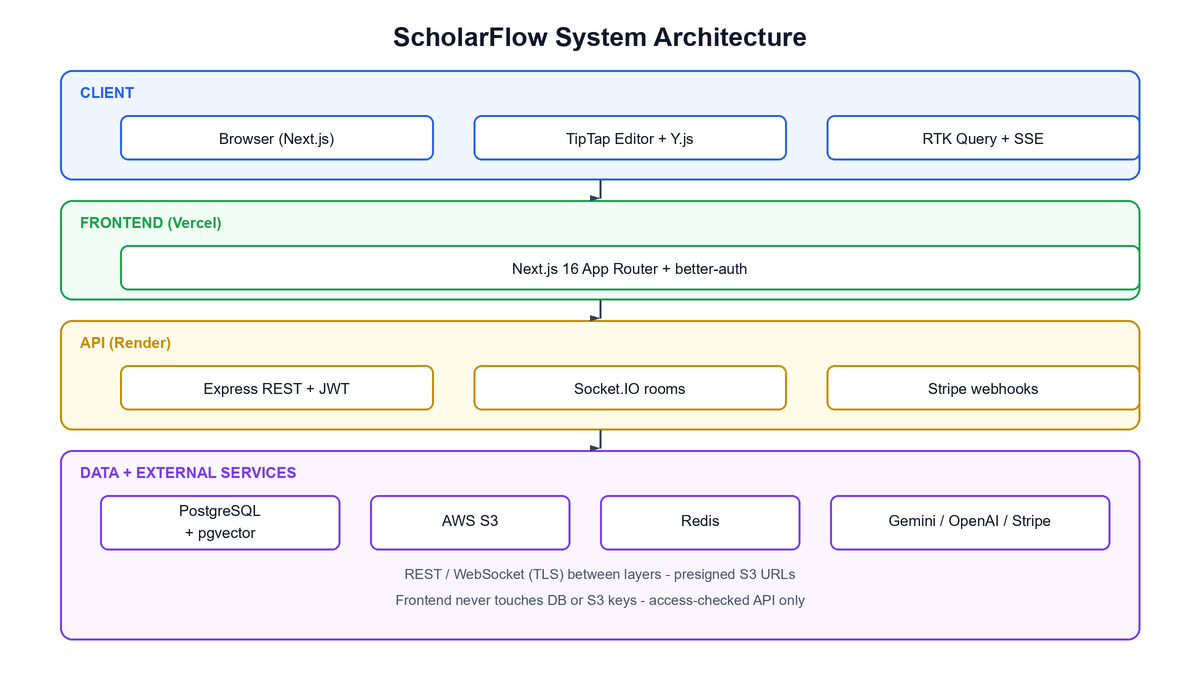
\includegraphics[width=0.95\textwidth]{figures/architecture.png}
\caption{ScholarFlow system architecture overview}
\label{fig:architecture}
\end{figure}

\subsection{Frontend Technologies}
Next.js 16 (App Router, Turbopack), React 19.2 + React Compiler (no manual
memoization), TypeScript strict, Tailwind CSS + shadcn/ui, RTK Query (all API
traffic; no raw fetch in components), React Hook Form + Zod, TipTap with
resizable-image, Y.js + socket.io client, Sonner toasts via provider helpers only.

\subsection{Backend Technologies}
Node.js $\geq$22, Express with TypeScript, strict Zod request validation,
thin controllers delegating to service-layer business logic, JWT with
bcrypt and refresh token rotation, rate limiting on mutations, Stripe SDK
for subscriptions and webhooks, Resend and SMTP email delivery, an hourly
node-cron sweeper, and Socket.IO rooms with JWT authentication.

\subsubsection{Backend File Structure}
The backend follows a modular feature architecture under \texttt{src/app/modules/}, isolating controllers, services, routes, and validation schemas:

\begin{verbatim}
backend/src/app/
|-- modules/
|   |-- Auth/         % JWT auth, bcrypt hashing, token rotation
|   |-- User/         % Profile management, credentials, preferences
|   |-- papers/       % Upload, S3 presigned URLs, metadata extraction
|   |-- annotations/  % PDF highlight marks, colors, and notes
|   |-- Workspace/    % Multi-tenant spaces, member roles, invitations
|   |-- Team/         % Lab collaborator management, role permissions
|   |-- AI/           % Multi-model LLM routing (Gemini/OpenAI/Claude)
|   |-- Search/       % pgvector HNSW cosine similarity search
|   |-- Billing/      % Stripe checkout, webhooks, portal, sweeper
|   |-- WebSocket/    % Socket.IO rooms, Y.js document synchronization
|   |-- Notification/ % Real-time SSE push streams, quiet hours
|   `-- Admin/        % System telemetry, user moderation, audit logs
|-- middleware/       % JWT verification, RBAC guards, rate limiters
`-- routes/           % Centralized REST route registration
\end{verbatim}

\subsection{Database Architecture}
Single shared PostgreSQL (Prisma Cloud) for dev and production; Prisma 7.8.0
with \texttt{@prisma/adapter-pg} pooling. Core ER model in
Fig.~\ref{fig:erd}: auth (User/Account/Session), collaboration
(Workspace/Member), library (Paper/File/Chunk, Collection), AI artifacts
(summaries, insight threads, embeddings). pgvector HNSW index
(\texttt{vector\_cosine\_ops}, m=16, ef\_construction=64); typed raw SQL only
for vector ops; one statement per file under \texttt{prisma/sql/}.

\begin{figure}[H]
\centering
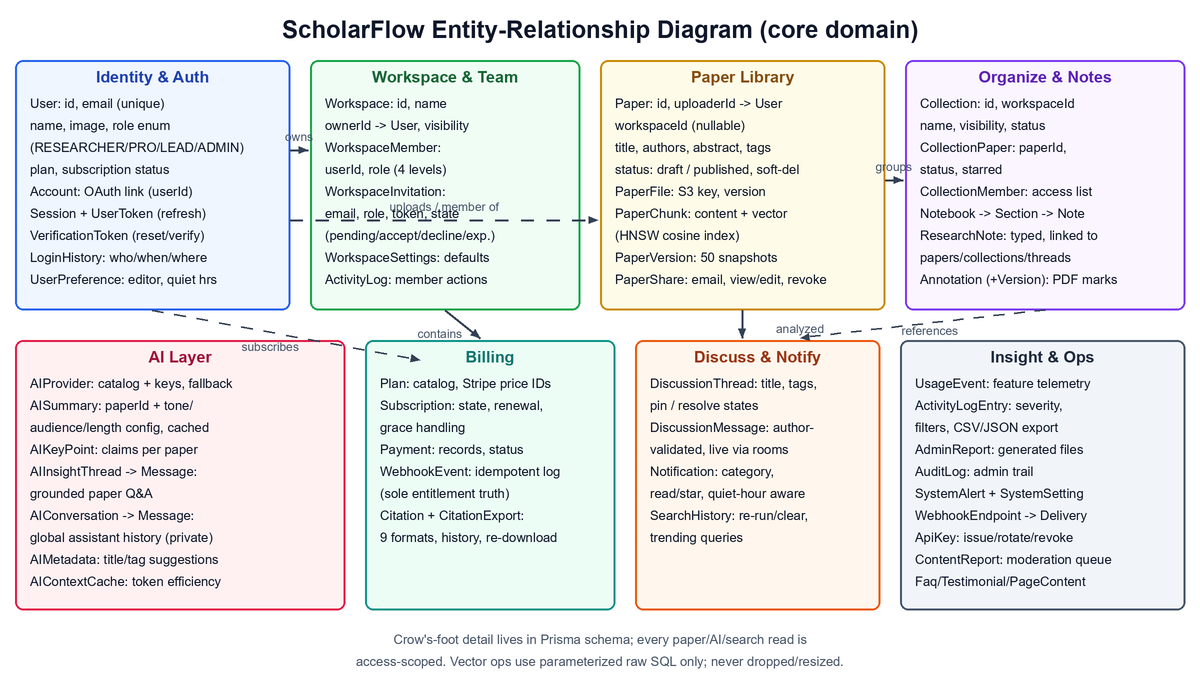
\includegraphics[width=0.95\textwidth]{figures/erd.png}
\caption{Entity--relationship diagram: full core domain (8 groups)}
\label{fig:erd}
\end{figure}

\subsection{AI and Machine Learning Integration}
Multi-provider service (Gemini primary, OpenAI/Claude/DeepSeek fallback),
embeddings pipeline with fixed-dimension validation and chunking, RAG-style
Q\&A over paper chunks, token-efficient context caching. Paper lifecycle in
Fig.~\ref{fig:lifecycle}.

\begin{figure}[H]
\centering
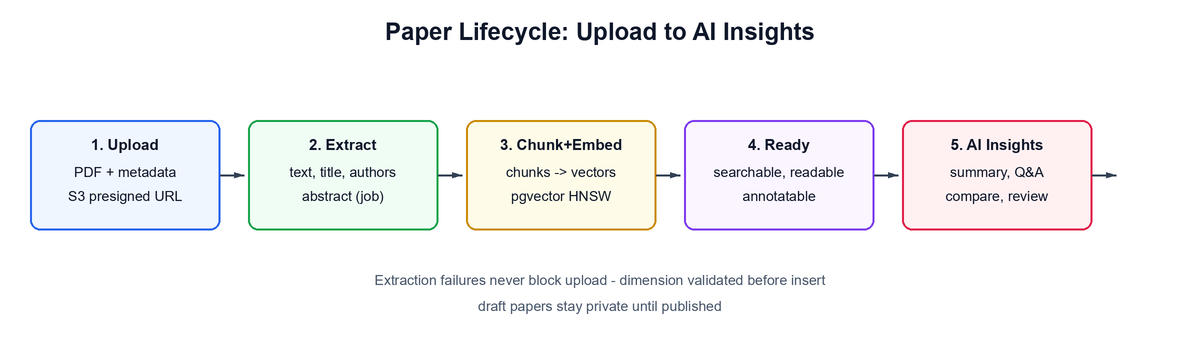
\includegraphics[width=0.9\textwidth]{figures/paper_lifecycle.png}
\caption{Paper lifecycle: upload, extraction, indexing, AI insights}
\label{fig:lifecycle}
\end{figure}

\subsection{Real-Time Communication Layer}
Dedicated Socket.IO server (Render) + in-app setup: JWT-verified handshake,
per-paper/discussion/workspace rooms, Y.js document sync, cursor presence,
typing indicators, late-joiner state sync, REST fallback when offline.

\subsection{Authentication and Security Architecture}
better-auth on the frontend paired with backend JWT authentication; OAuth
never overwrites user-customized profile names or avatars; RBAC via
\texttt{requireRole} after auth middleware; per-resource ownership checks in
services; presigned S3 URLs only; verified Stripe webhooks; admin-gated
metrics and team member search.

\subsection{External Integrations}
Google/GitHub OAuth, Gemini/OpenAI/Claude/DeepSeek AI, AWS S3, Stripe,
Resend/SMTP email, OpenAlex/arXiv scholarly feeds (TTL-cached, graceful
degradation).

\subsection{DevOps and Deployment Architecture}
Turborepo + Yarn Berry monorepo; Vercel (frontend), Render (API + socket
server); same Prisma Postgres for local and prod; GitHub Actions CI
(test + lint + type-check + build); health endpoints
(\texttt{/api/health}, \texttt{/detailed}, \texttt{/live}, \texttt{/ready}).

\subsection{Development and Testing Tools}
Jest + Supertest (21 suites / 59 tests, green), Playwright E2E, ESLint flat
configs, Prettier, Prisma Studio, Stripe CLI webhook forwarding, Repomix
snapshots.

\subsection{Key Technical Highlights}
\begin{itemize}[nosep]
\item Decoupled monorepo: frontend never imports backend/Prisma; REST only.
\item $<$50\,ms server-side query budget with slow-query terminal visibility.
\item Idempotent billing webhooks + sweeper (never webhook-only downgrades).
\item WCAG 2.1 AA, responsive 375\,px--desktop, dark mode.
\end{itemize}
